\documentclass[aspectratio=169, 10pt]{beamer}

\usepackage{bm} % bold math
\usepackage{fontspec}
\usepackage{minted}
\usepackage{pgf-pie}
\usepackage{tikz}
\usepackage{graphicx}
\newcommand\sbullet[1][.5]{\mathbin{\vcenter{\hbox{\scalebox{#1}{$\bullet$}}}}}

% Custom commands and environments
\makeatletter
\newcommand\version[1]{\renewcommand\@version{#1}}
\newcommand\@version{}
\def\insertversion{\@version}

\newcommand\course[1]{\renewcommand\@course{#1}}
\newcommand\@course{}
\def\insertcourse{\@course}

\newcommand\coursetitle[1]{\renewcommand\@coursetitle{#1}}
\newcommand\@coursetitle{}
\def\insertcoursetitle{\@coursetitle}

\newcommand\lecturenumber[1]{\renewcommand\@lecturenumber{#1}}
\newcommand\@lecturenumber{}
\def\insertlecturenumber{\@lecturenumber}
\makeatother

\newcommand{\slidetitle}[1]{{\xbseries \large \structure{#1}} \bigskip}
\newcommand{\term}[1]{{\color{blue} #1}}
\newcommand{\leftspace}{\hspace{1em}}
\newcommand{\inlinearrow}{
  
\begin{tikzpicture}[baseline]
    \node [anchor=base] (x) {};
    \draw [rawarrow] (x.mid west) -- ($(x.mid west) + (2em,0)$);
  \end{tikzpicture}
}

\newenvironment{slide}
{\begin{frame}[fragile,environment=slide]\vskip0pt plus 1filll}
{\vskip0pt plus 1filll\end{frame}}

% LaTeX

\setlength{\leftmargini}{1em}

% Common Information

\author{Talia Xu}
\course{COMPSCI 340}
\coursetitle{Operating Systems}
\date{2024 Semester 2}

% fontspec

\defaultfontfeatures{Ligatures=TeX}
% \setmainfont{Domine}
\setsansfont{Inter}[
  FontFace={ul}{n}{Font=*-Thin},
  FontFace={el}{n}{Font=*-ExtraLight},
  FontFace={l}{n}{Font=*-Light},
  FontFace={sb}{n}{Font=*-SemiBold},
  FontFace={eb}{n}{Font=*-ExtraBold},
  FontFace={xb}{n}{Font=*-Black},
]
\setmonofont[Contextuals=AlternateOff, Ligatures=TeXOff]{Iosevka}[
  FontFace={xb}{n}{Font=*-Heavy},
]

%% Font Weights

\DeclareRobustCommand{\ulseries}{\fontseries{ul}\selectfont}
\DeclareTextFontCommand{\textul}{\ulseries}
\DeclareRobustCommand{\elseries}{\fontseries{el}\selectfont}
\DeclareTextFontCommand{\textel}{\elseries}
\DeclareRobustCommand{\lseries}{\fontseries{l}\selectfont}
\DeclareTextFontCommand{\textl}{\lseries}
\DeclareRobustCommand{\sbseries}{\fontseries{sb}\selectfont}
\DeclareTextFontCommand{\textsb}{\sbseries}
\DeclareRobustCommand{\ebseries}{\fontseries{eb}\selectfont}
\DeclareTextFontCommand{\texteb}{\ebseries}
\DeclareRobustCommand{\xbseries}{\fontseries{xb}\selectfont}
\DeclareTextFontCommand{\textxb}{\xbseries}

% tikz

\usetikzlibrary{
  arrows,
  arrows.meta,
  automata,
  backgrounds,
  calc,
  decorations.pathreplacing,
  matrix,
  positioning,
  overlay-beamer-styles,
  shapes,
  shapes.multipart,
  tikzmark,
}

\tikzstyle{rawarrow} = [
  -{Latex[round]},
  line width=1pt,
  yellow,
  shorten >=3pt,
  shorten <=3pt,
  font=\small,
  text=black,
]

\tikzstyle{arrow} = [
  -{Latex[round]},
  line width=1pt,
  yellow,
  shorten >=3pt,
  shorten <=3pt,
  transform canvas={yshift=3pt},
  font=\small,
  text=black,
]

\newcommand{\tikzmarkcoord}[1]{([yshift=3pt]pic cs:#1)}

% minted

\setminted{style=eyolfson, fontsize=\small, escapeinside=||}
\setmintedinline{fontsize=\normalsize}

% hyperref

\hypersetup{colorlinks, urlcolor=blue}

% beamer
\setbeamersize{text margin left=16mm, text margin right=16mm}
\setbeamertemplate{itemize items}[circle]
\setbeamercolor{item}{fg=black}
\setbeamercolor{structure}{fg=darkblue}
\setbeamerfont{frametitle}{series=\bfseries, parent=structure}
\setbeamertemplate{navigation symbols}{}
\setbeamertemplate{headline}{}
\setbeamertemplate{footline}{
  \begin{tikzpicture}[
    remember picture,
    overlay,
    shift={(current page.south west)},
  ]
    \path [fill=gray] (144mm, 0) -- (160mm, 16mm) -- (160mm, 0);
    \node [inner sep=3.5mm, outer sep=0, text=black, anchor=base east,
           align=right, yshift=3.5mm]
          at (current page.south east) {\ttfamily \small \insertframenumber{}};
  \end{tikzpicture}
}
\setbeamertemplate{title page}{
  \begin{tikzpicture}[
    remember picture,
    overlay,
    shift={(current page.south west)},
    background rectangle/.style={fill=darkblue},
    show background rectangle,
  ]
    \node [anchor=center, align=center, text=white, text width=40mm, scale=3.2]
          at (\paperwidth / 2, \paperheight * 2 / 3)
          {\xbseries \inserttitle{}};
    \node [anchor=base west, align=left, inner sep=0, text=white, yshift=2.5mm]
          at (16mm, \paperheight / 3)
          {\insertdate{} \insertcourse{}: \insertcoursetitle{}};
    \node [anchor=base west, align=left, inner sep=0, text=white, yshift=-2.5mm]
          at (16mm, \paperheight / 3)
          {\insertauthor};
    \node [anchor=base east, align=right, inner sep=0, text=white, yshift=2.5mm]
          at (144mm, \paperheight / 3)
          {Lecture \insertlecturenumber{}};
    \node [anchor=base east, align=right, inner sep=0, text=white,
           yshift=-2.5mm]
          at (144mm, \paperheight / 3)
          {\ttfamily \insertversion{}};
    \node [align=center, anchor=south, inner sep=0, text=white, yshift=3.5mm]
          (license) at (\paperwidth / 2, 0)
          {\fontsize{7pt}{7pt}\selectfont This  work is licensed under a
           \href{http://creativecommons.org/licenses/by-sa/4.0/}
                {\color{lightblue} Creative Commons Attribution-ShareAlike 4.0
                 International License}};
  \end{tikzpicture}
}

% xcolor

%% Primary Colour

\definecolor{pantone655}{RGB}{0, 42, 92} % #002a5c
\colorlet{darkblue}{pantone655}

%% Secondary Colours

\definecolor{pantone633}{RGB}{0, 139, 176} % #008bb0
\colorlet{blue}{pantone633}

\definecolor{pantonewarmred}{RGB}{220, 70, 51} % #dc4633
\colorlet{red}{pantonewarmred}

\definecolor{pantone3285}{RGB}{0, 161, 137} % #00a189
\colorlet{cyan}{pantone3285}

\definecolor{pantone7722}{RGB}{13, 83, 77} % #0d534d
\colorlet{darkcyan}{pantone7722}

\definecolor{pantone376}{RGB}{141, 191, 46} % #8dbf2e
\colorlet{green}{pantone376}

\definecolor{pantone2613}{RGB}{109, 36, 122} % #6d247a
\colorlet{violet}{pantone2613}

\definecolor{pantone2985}{RGB}{111, 199, 234} % #6fc7ea
\colorlet{lightblue}{pantone2985}

\definecolor{pantone227}{RGB}{171, 19, 104} % #ab1368
\colorlet{magenta}{pantone227}

\definecolor{pantone7406}{RGB}{241, 197, 0} % #f1c500
\colorlet{yellow}{pantone7406}

%% Neutrals

\definecolor{pantonecoolgray2}{RGB}{208, 209, 201} % #d0d1c9
\colorlet{gray}{pantonecoolgray2}


\lecturenumber{10}
\title{Advanced Scheduling}
\version{2.0.0}

\begin{document}
  \begin{frame}[plain, noframenumbering]
    \titlepage
  \end{frame}

  \begin{slide}

    \slidetitle{We Could Add Priorities}

    We may favor some processes over others

    \leftspace{}Assign each process a priority
    \medskip

    Run higher priority processes first, round-robin processes of equal priority

    \leftspace{}Can be preemptive or non-preemptive

  \end{slide}

  \begin{slide}

    \slidetitle{Priorities Can Be Assigned an Integer}

    We can pick a lower, or higher number, to mean high priority

    \leftspace{}In Linux -20 is the highest priority, 19 is the lowest
    \medskip

    We may lead processes to \textit{starvation} if there's a lot of higher
    priority processes
    \medskip

    One solution is to have the OS dynamically change the priority

    \leftspace{}Older processes that haven't been executed in a long time increase priority

  \end{slide}

  \begin{slide}

    \slidetitle{Priority Inversion is a New Issue}

    We can accidentally change the priority of a low priority process to a high one

    \leftspace{}This is caused by dependencies, e.g. a high priority depends a low priority
    \medskip

    One solution is \textit{priority inheritance}

    \leftspace{}Inherit the highest priority of the waiting processes

    \leftspace{}Chain together multiple inheritances if needed

    \leftspace{}Revert back to the original priority after dependency

  \end{slide}

  \begin{slide}

    \slidetitle{A Foregound Process Can Recieve User Input, Background Can Not}

    Unix background process when: process group ID differs from its terminal group ID

    \leftspace{}You do not need to know this specific definition
    \medskip

    The idea is to separate processes that users interact with:

    \leftspace{}Foreground processes are interactable and need good response time

    \leftspace{}Background processes may not need good response time, just throughput

  \end{slide}

  \begin{slide}

    \slidetitle{We Can Use Multiple Queues for Other Purposes}

    We could create different queues for foreground and background processes:

    \leftspace{}Foreground uses RR

    \leftspace{}Background uses FCFS
    \medskip

    Now we have to schedule between queues!

    \leftspace{}RR between the queues

    \leftspace{}Use a priority for each queue

  \end{slide}

  \begin{slide}

    \slidetitle{Scheduling Can Get Complicated}

    There's no ``right answer'', only trade-offs
    \medskip

    We haven't talked about multiprocessor scheduling yet
    \medskip

    We'll assume symmetric multiprocessing (SMP)

    \leftspace{}All CPUs are connected to the same physical memory

    \leftspace{}The CPUs have their own private cache (at least the lowest levels)

  \end{slide}

  \begin{slide}

    \slidetitle{One Approach is to Use the Same Scheduling for All CPUs}

    There's still only one scheduler

    \leftspace{}It just keeps adding processes while there's available CPUs
    \medskip

    Advantages

    \leftspace{}Good CPU utilization

    \leftspace{}Fair to all processes
    \medskip

    Disadvantages

    \leftspace{}Not scalable (everything blocks on global scheduler)

    \leftspace{}Poor cache locality
    \medskip

    This was the approach in Linux 2.4

  \end{slide}

  \begin{slide}

    \slidetitle{We Can Create Per-CPU Schedulers}

    When there's a new process, assign it to a CPU

    \leftspace{}One strategy is to assign it to the CPU with the lowest number of processes
    \medskip

    Advantages

    \leftspace{}Easy to implement

    \leftspace{}Scalable (there's no blocking on a resource)

    \leftspace{}Good cache locality
    \medskip

    Disadvantages

    \leftspace{}Load imbalance

    \leftspace{}\leftspace{}Some CPUs may have less processes, or less intensive ones

  \end{slide}

  \begin{slide}

    \slidetitle{We Can Compromise between Global and Per-CPU}

    Keep a global scheduler that can rebalance per-CPU queues

    \leftspace{}If a CPU is idle, take a process from another CPU (work stealing)
    \medskip

    You may want more control over which processes can switch

    \leftspace{}Some may be more sensitive to caches
    \medskip

    Use \textit{processor affinity}

    \leftspace{}The preference of a process to be scheduled on the same core
    \medskip

    This is a simplified version of the O(1) scheduler in Linux 2.6

  \end{slide}

  \begin{slide}

    \slidetitle{Another Strategy is ``Gang'' Scheduling}

    Multiple processes may need to be scheduled simultaneously
    \medskip

    The scheduler on each CPU cannot be completely independent
    \medskip

    ``Gang Scheduling'' (Coscheduling)

    \leftspace{}Allows you to run a set of processes simultaneously (acting as a unit)
    \medskip

    This requires a global context-switch across all CPUs

  \end{slide}

  \begin{slide}

    \slidetitle{Real-Time Scheduling is Yet Another Problem}

    Real-time means there are time constraints, either for a deadline or rate

    \leftspace{}e.g. audio, autopilot
    \medskip

    A hard real-time system

    \leftspace{}Required to guarantee a task completes within a certain amount
    of time
    \medskip

    A soft real-time system

    \leftspace{}Critical processes have a higher priority and the deadline is
    met in practice
    \medskip

    Linux is an example of soft real-time

  \end{slide}

  \begin{slide}

    \slidetitle{Linux Also Implements FCFS and RR Scheduling}

    You can search the source tree: FCFS (\texttt{SCHED\_FIFO}) and RR (\texttt{SCHED\_RR})
    \medskip

    Use a multilevel queue scheduler for processes with the same priority

    \leftspace{}Also let the OS dynamically adjust the priority
    \medskip

    Soft real-time processes:

    \leftspace{}Always schedule the highest priority processes first
    \medskip

    Normal processes:

    \leftspace{}Adjust the priority based on aging

  \end{slide}

  \begin{slide}

    \slidetitle{Real-Time Processes Are Always Prioritized}

    The soft real-time scheduling policy will either be \texttt{SCHED\_FIFO}
    or \texttt{SCHED\_RR}

    \leftspace{}There are 100 static priority levels (0---99)
    \medskip

    Normal scheduling policies apply to the other processes
    (\texttt{SCHED\_NORMAL})

    \leftspace{}By default the priority is 0

    \leftspace{}Priority ranges from $\mathsf{[-20, 19]}$
    \medskip

    Processes can change their own priorities with system calls:

    \leftspace{}\texttt{nice}, \texttt{sched\_setscheduler}

  \end{slide}

  \begin{slide}
    
    \slidetitle{Linux Priority Unifies Soft Real-time and Normal Processes}

    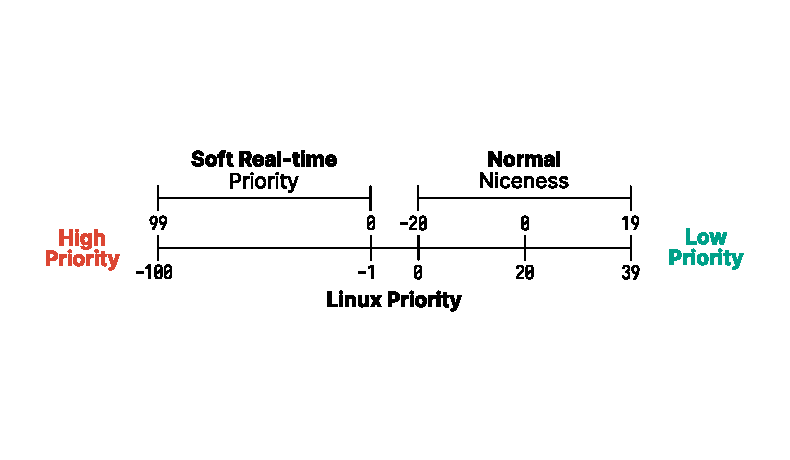
\includegraphics{linux-priority.eps}

  \end{slide}

  \begin{slide}

    \slidetitle{Linux Scheduler Evolution}

    2.4---2.6, a $\mathsf{O(N)}$ global queue

    \leftspace{}Simple, but poor performance with multiprocessors and many processes
    \medskip

    2.6---2.6.22, a per-CPU run queue, $\mathsf{O(1)}$ scheduler

    \leftspace{}Complex to get right, interactivity had issues

    \leftspace{}No guarantee of fairness
    \medskip

    2.6.23---Present, the completely fair scheduler (CFS)

    \leftspace{}Fair, and allows for good interactivity

  \end{slide}

  \begin{slide}

    \slidetitle{The $\mathsf{O(1)}$ Scheduler Has Issues with Modern Processes}

    Foreground and background processes are a good division

    \leftspace{}Easier with a terminal, less so with GUI processes
    \medskip

    Now the kernel has to detect interactive processes with heuristics

    \leftspace{}Processes that sleep a lot may be more interactive

    \leftspace{}\leftspace{}This is ad hoc, and could be unfair
    \medskip

    How would we introduce fairness for different priority processes?

    \leftspace{}Use different size time slices

    \leftspace{}The higher the priority, the larger the time slice

    \leftspace{}\leftspace{}There are also situations where this ad hoc solution
    could be unfair

  \end{slide}

  \begin{slide}

    \slidetitle{Ideal Fair Scheduling}

    Assume you have an infinitely small time slice

    \leftspace{}If you have $\mathsf{n}$ processes, each runs at $\mathsf{\frac{1}{n}}$ rate
    \medskip

    \begin{tikzpicture}
      \draw (0, 6em) rectangle (30em, 7.5em);

      \node [anchor=east] at (0, 6.75em) {1 Process};

      \draw (0, 3.5em) rectangle (10em, 5em);
      \draw (0, 1.75em) rectangle (10em, 3.25em);
      \draw (0, 0) rectangle (10em, 1.5em);

      \node [anchor=east] at (0, 2.5em) {3 Processes};
    \end{tikzpicture}
    \bigskip

    CPU usage is divided equally among every process

  \end{slide}

  \begin{slide}

    \slidetitle{Example IFS Scheduling}

    Consider the following processes:

    \begin{center}
      \footnotesize
      \begin{tabular}{lrr}
        Process & Arrival Time & Burst Time \\
        $\mathsf{P_1}$ & 0 & 8 \\
        $\mathsf{P_2}$ & 0 & 4 \\
        $\mathsf{P_3}$ & 0 & 16 \\
        $\mathsf{P_4}$ & 0 & 4 \\
      \end{tabular}
    \end{center}

    Assume that each vertical slice can execute 4 time units.

    \leftspace{}Each box represents the time units spend executing

    \begin{center}
      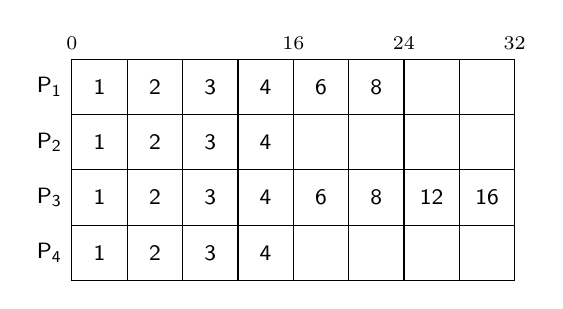
\begin{tikzpicture}

        %% \fill [black!80] (0,0) rectangle (14em, 2em);

        %% \fill [black!60] (14em,0) rectangle (22em, 2em);

        %% \fill [black!40] (22em,0) rectangle (24em, 2em);

        %% \fill [black!20] (24em,0) rectangle (32em, 2em);

        \draw (0,0) rectangle (16em,8em);

        \foreach \i in {1,...,7} {
          \draw [shorten >=0] (\i * 2em, 0) -- (\i * 2em, 8em);
        }

        \foreach \i in {1,...,3} {
          \draw [shorten >=0] (0, \i * 2em) -- (16em, \i * 2em);
        }

        \node [anchor=east] at (0, 7em) {\footnotesize $\mathsf{P_1}$};
        \node [anchor=east] at (0, 5em) {\footnotesize $\mathsf{P_2}$};
        \node [anchor=east] at (0, 3em) {\footnotesize $\mathsf{P_3}$};
        \node [anchor=east] at (0, 1em) {\footnotesize $\mathsf{P_4}$};

        \node at (1em, 7em) {\footnotesize $\mathsf{1}$};
        \node at (1em, 5em) {\footnotesize $\mathsf{1}$};
        \node at (1em, 3em) {\footnotesize $\mathsf{1}$};
        \node at (1em, 1em) {\footnotesize $\mathsf{1}$};

        \node at (3em, 7em) {\footnotesize $\mathsf{2}$};
        \node at (3em, 5em) {\footnotesize $\mathsf{2}$};
        \node at (3em, 3em) {\footnotesize $\mathsf{2}$};
        \node at (3em, 1em) {\footnotesize $\mathsf{2}$};

        \node at (5em, 7em) {\footnotesize $\mathsf{3}$};
        \node at (5em, 5em) {\footnotesize $\mathsf{3}$};
        \node at (5em, 3em) {\footnotesize $\mathsf{3}$};
        \node at (5em, 1em) {\footnotesize $\mathsf{3}$};

        \node at (7em, 7em) {\footnotesize $\mathsf{4}$};
        \node at (7em, 5em) {\footnotesize $\mathsf{4}$};
        \node at (7em, 3em) {\footnotesize $\mathsf{4}$};
        \node at (7em, 1em) {\footnotesize $\mathsf{4}$};

        \node at (9em, 7em) {\footnotesize $\mathsf{6}$};
        \node at (9em, 3em) {\footnotesize $\mathsf{6}$};

        \node at (11em, 7em) {\footnotesize $\mathsf{8}$};
        \node at (11em, 3em) {\footnotesize $\mathsf{8}$};

        \node at (13em, 3em) {\footnotesize $\mathsf{12}$};

        \node at (15em, 3em) {\footnotesize $\mathsf{16}$};

        \node [anchor=south] at (0em, 8em) {\scriptsize 0};
        \node [anchor=south] at (8em, 8em) {\scriptsize 16};
        \node [anchor=south] at (12em, 8em) {\scriptsize 24};
        \node [anchor=south] at (16em, 8em) {\scriptsize 32};
      \end{tikzpicture}
    \end{center}

  \end{slide}

  \begin{slide}

    \slidetitle{IFS is the Fairest but Impractical Policy}

    This policy is fair, every process gets an equal amount of CPU time

    \leftspace{}Boosts interactivity, has the ideal response time
    \medskip

    However, this would perform way too many context switches
    \medskip

    You have to constantly scan all processes, which is $\mathsf{O(N)}$

  \end{slide}

  \begin{slide}

    \slidetitle{Completely Fair Scheduler (CFS)}

    For each runnable process, assign it a ``virtual runtime''

    \leftspace{}At each scheduling point where the process runs for time \texttt{t}

    \leftspace{}\leftspace{}Increase the virtual runtime by \texttt{t}
    $\mathsf{\times}$ weight (based on priority)
    \medskip

    The virtual runtime monotonically increases

    \leftspace{}Scheduler selects the process based on the lowest virtual runtime

    \leftspace{}\leftspace{}Compute its dynamic time slice based on the IFS
    \medskip

    Allow the process to run, when the time slice ends repeat the process

  \end{slide}

  \begin{slide}

    \slidetitle{CFS is Implemented with Red-Black Trees}

    A red-black tree is a self-balancing binary search tree

    \leftspace{}Keyed by virtual runtime

    \leftspace{}\leftspace{}$\mathsf{O(lg N)}$ insert, delete, update, find
    minimum
    \medskip

    The implementation uses a red-black tree with nanosecond granularity

    \leftspace{}Doesn't need to guess the interactivity of a process
    \medskip

    CFS tends to favour I/O bound processes by default

    \leftspace{}Small CPU bursts translate to a low virtual runtime

    \leftspace{}\leftspace{}It will get a larger time slice, in order to catch
    up to the ideal

  \end{slide}

  \begin{slide}

    \slidetitle{Scheduling Gets Even More Complex}

    There are more solutions, and more issues:

    \begin{itemize}
      \item Introducing priority also introduces priority inversion
      \item Some processes need good interactivity, others not so much
      \item Multiprocessors may require per-CPU queues
      \item Real-time requires predictability
      \item Completely Fair Scheduler (CFS) tries to model the ideal fairness
    \end{itemize}

  \end{slide}

\end{document}
